\documentclass[letterpaper]{article}
\usepackage{aaai}
\usepackage{times}
\usepackage{helvet}
\usepackage{courier}
\usepackage{graphicx}
\usepackage{url}
\usepackage{fancyvrb}

\newcommand{\citenoun}[1]{\citeauthor{#1}~\shortcite{#1}}
\newcommand{\citenounpg}[2]{\citeauthor{#2}~\shortcite[#1]{#2}}

\title{Prototyping Games with BIPED}

%\author{Demo (paper \#34)\\
%Keywords: game design, logic, scripting
%}
\author{Adam M. Smith$^\star$, Mark J. Nelson$^{\star\dagger}$, Michael Mateas$^\star$\\
$^\star$ Expressive Intelligence Studio, University of California, Santa Cruz\\
$^\dagger$ School of Interactive Computing, Georgia Institute of Technology\\
\texttt{amsmith@cs.ucsc.edu, mnelson@cc.gatech.edu, michaelm@cs.ucsc.edu}
}
\copyrightyear{2009}

\begin{document}
\maketitle

\begin{abstract}

We demonstrate the use of BIPED, a system that explores a new approach to
supporting the early stages of game design. Using BIPED, a game designer can
leverage a single, concise game definition to get both a playable prototype and
a formal rule system. In this way, BIPED's two legs give a designer access to
insight: the first through feedback from human players (revealing player
hesitation, engagement, or fun) and the second through automated analysis
(revealing emergent properties, exploits, and puzzle solutions).

Our system focuses on board-game-like prototypes. On screen, human players
manipulate individual tokens that are arranged on board spaces linked by paths.
Using the mouse, they can trigger game events that interact with the
designer-specified game mechanics. On the design side, designers have access to
timers, allowing them to create interesting, real-time dynamics.

In addition to play testing with human subjects, we support a form of machine
play testing. Using only the game definition, our analysis engine is capable
of imagining complete play traces showing a log of game state and events over
time. To drill down on interesting scenarios, the designer may specify
additional constraints and ask the engine to show only (and possibly all)
traces that fit these constraints. Examples include: defeat happens at time
seven, no more than six monsters are slain, and the player character always
picks up treasures.

\end{abstract}

\section{Introduction}

\begin{figure}
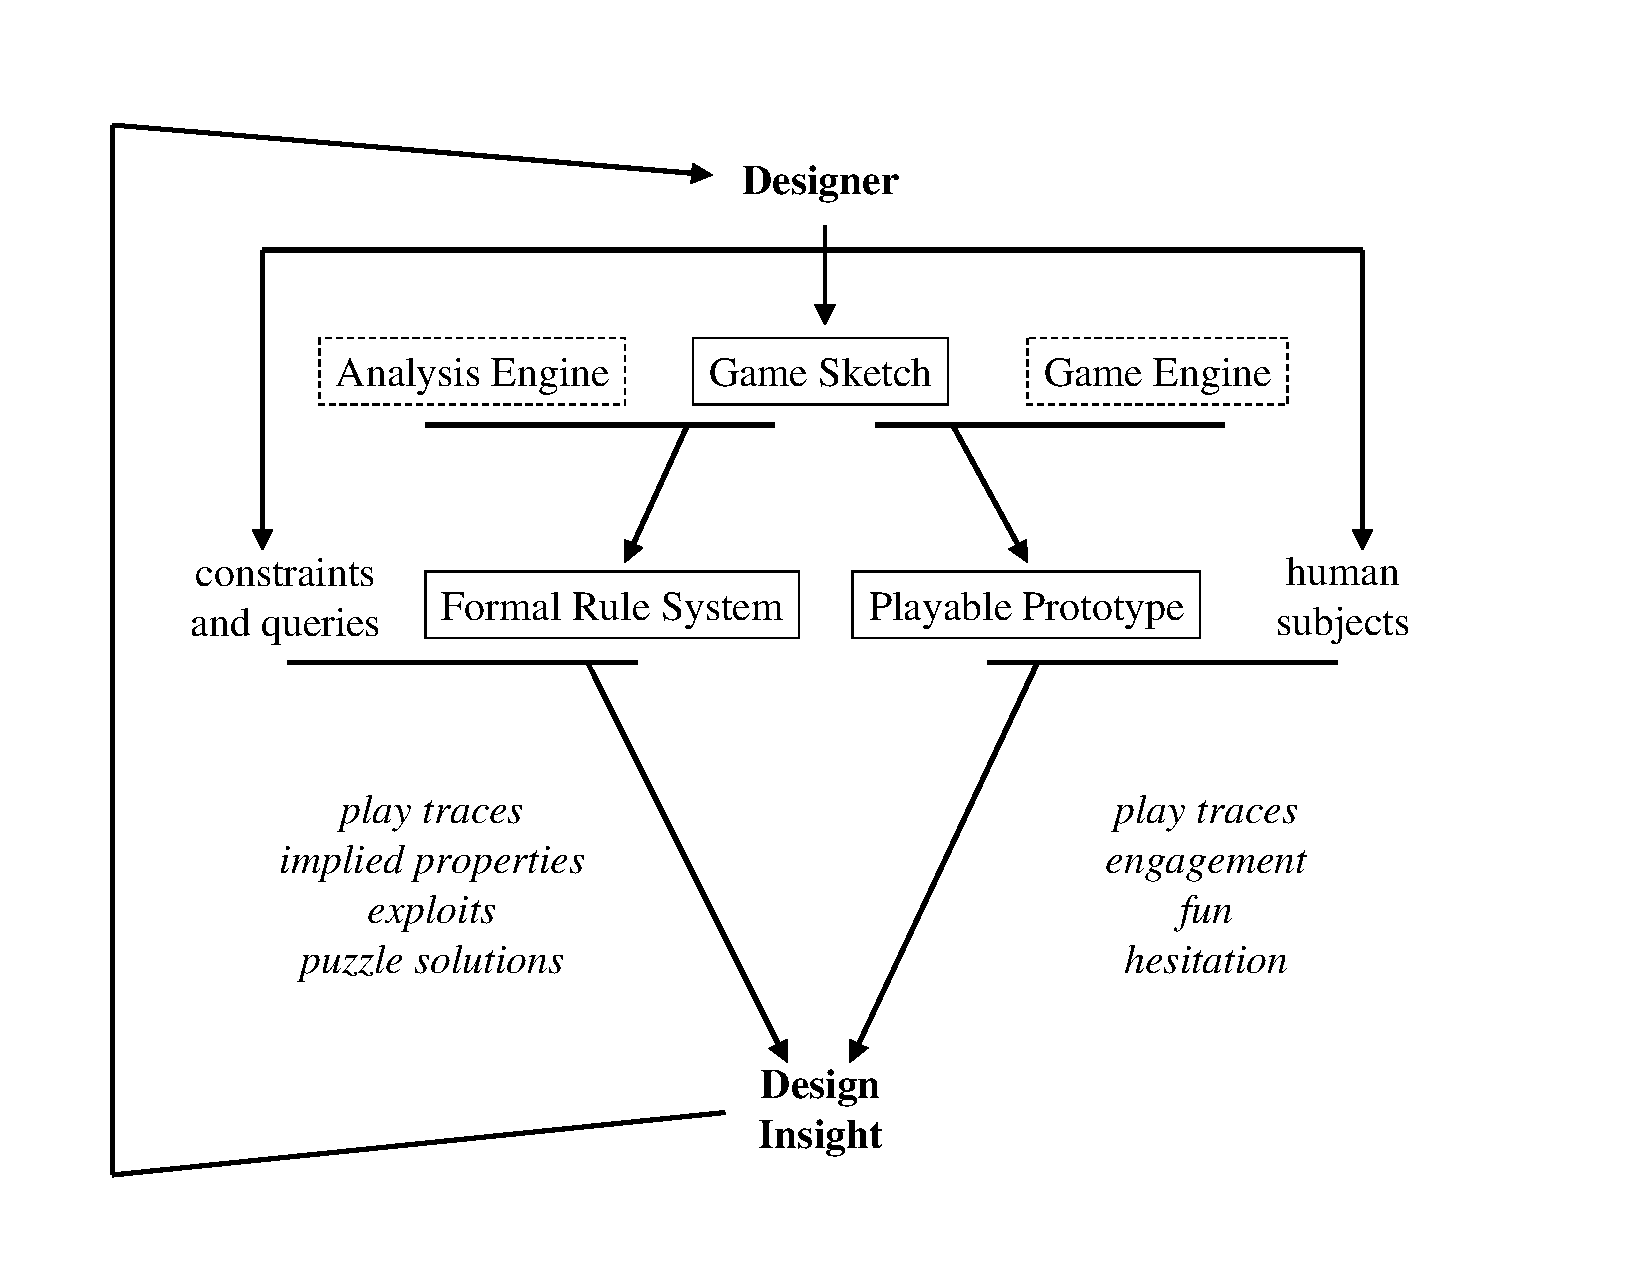
\includegraphics[viewport=0.5in 0.5in 9.5in 8in,clip,width=\columnwidth]{architecture.pdf}
\caption{Architecture diagram for the BIPED system.}
\label{fig:arch}
\end{figure}

\citenounpg{p.\ 248}{Fullerton} calls play testing ``the single most important
activity a designer engages in''. Our system, BIPED, focuses on providing
computational support for play testing early-stage game prototypes. Early-stage
prototypes are often built out of physical elements such as cards, tokens, or
dice, the same elements used in board games. BIPED provides a game-sketching
language that a designer can use to quickly prototype a game idea using
on-screen versions of these kinds of representational elements. A more complete
overview is given in the accompanying full paper~\cite{BIPEDfull}.

Game sketches created with BIPED support human play testing by producing 
computational prototypes. With these prototypes, the designer can
carry out traditional play testing.  Ideally, BIPED would be used after initial
play testing with a physical prototype (which gives the designer experience
with the game's foundation using soft, negotiable rules), but before the
implementation of a detailed computational prototype that may be more difficult
to iterate on in response to feedback.

Unique to BIPED prototypes is the ability to carry out machine play testing
using the same game-sketch definition that human players play. For us,
machine play testing means extracting gameplay traces with interesting
properties, using the analysis technique of \citenoun{NelsonMateas:AIIDE08}.
These traces can expose a difference between how the few human play testers
played and what a dedicated player might achieve with practice our brute-force
search. More importantly, these traces show how a game's mechanics work
immediately, without the need to rope in testers after each change.

The role of the designer and their game sketch, and this dual support for play
testing, is outlined in Figure~\ref{fig:arch}. Play testing is not only useful
for the designer to improve their games; \citenoun{Niedenthal:DiGRA}
explains how prototypes can also be used to communicate and advertise design
ideas, among other things. By virtue of BIPED's architecture, designers can
produce basic standalone games that can be shared with peers more easily than
physical prototypes or computational prototypes with extensive dependencies.
Even traces resulting from machine play testing can serve as a concise
proof that the design supports the intended player experience.

\section{Example prototype}

\begin{figure}
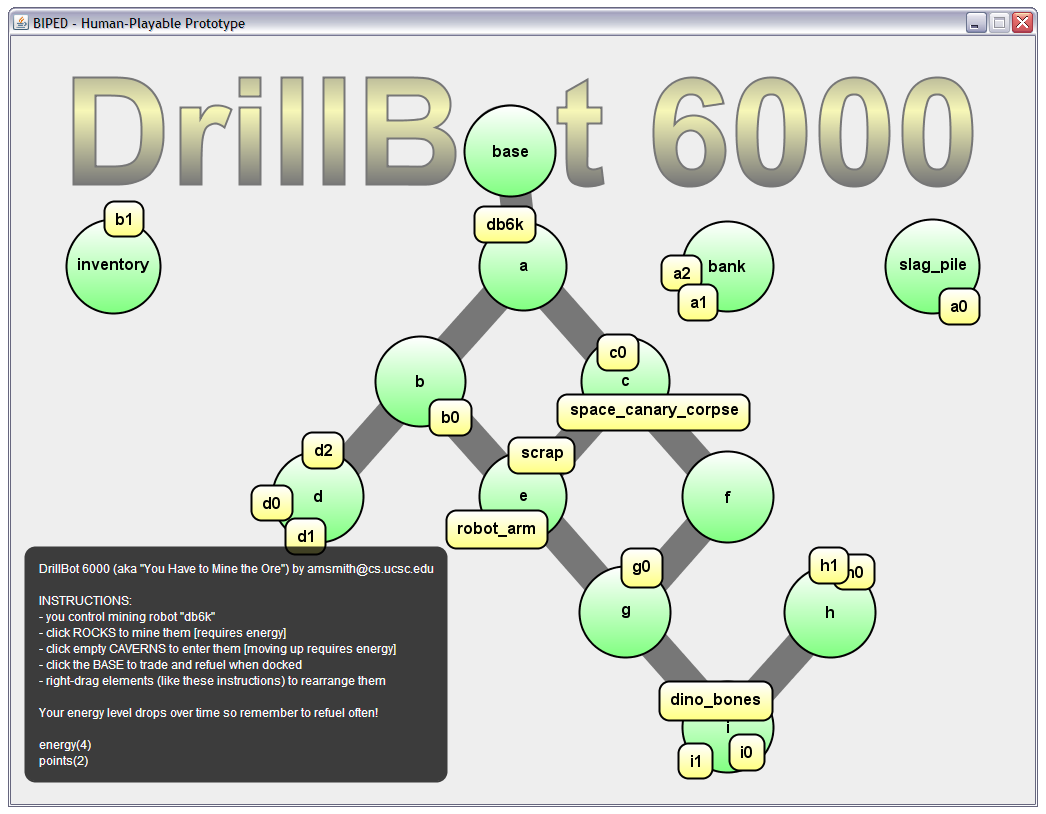
\includegraphics[width=\columnwidth]{db6k_screenshot.png}
\caption{\emph{DrillBot 6000}, a fast-paced mining game prototype, designed in
the style of \emph{Motherload}, powered by BIPED's game engine.}
\label{fig:screenshots}
\end{figure}

An example prototype in BIPED, \emph{DrillBot 6000}, is shown in Figure~\ref{fig:screenshots}.
\emph{DrillBot 6000} is a fast-paced mining game prototype based on
the core mechanics of the popular Flash game \emph{Motherload} from XGen
Studios.\footnote{\url{http://www.xgenstudios.com/play/motherload}} In this
game, the player moves a mining robot through underground caverns, drilling out
rocks of mixed value, while managing energy usage by periodically returning to
the surface to refuel and trade items. This game was relatively easy to sketch,
taking about 60 minutes of work to write 110 lines of game mechanics and 50
lines of UI bindings in our game-sketching language (not counting iterations
after play testing).

\section{Play testing}

We started play testing \emph{DrillBot 6000} using self-testing, briefly
playing the game ourselves to verify basic mechanics. Next, we tested with a
few human subjects. All three testers claimed to enjoy the game, and could
reach rocks at the deeper levels after some practice.  Interestingly, no
testers related to the game as a puzzle challenge, even when converted to a
turn-based mode; all focused instead on the action aspect.

Figure~\ref{fig:trace} shows an example gameplay trace from \emph{DrillBot
6000}, using the analysis engine, starting in the same scenario in which a
human player would start, and putting no particular constraints on traces.
From machine play testing, we learned that our human players were much more
cautious than the game's rules actually made necessary (frequently refueling
their robot). Other experiments revealed that one seemingly radical
level-design change did not affect either the maximum caverns reachable or the
maximum number of valuable rocks brought back in a fixed amount of time.

\begin{figure}
\begin{Verbatim}[frame=single,fontsize=\scriptsize]
happens( mine(a1), 0).
happens( drain, 1).
happens( drain, 2).
happens( trade, 3).
happens( refuel, 3).
happens( mine(a2), 4).
happens( mine(a0), 5).
happens( down_to(a), 6).
happens( mine(space_canary_corpse), 7).
happens( mine(c0), 8).
happens( down_to(c), 9).
happens( down_to(f), 10).
happens( up_to(c), 11).
happens( up_to(a), 12).
happens( down_to(c), 13).
happens( down_to(f), 14).
\end{Verbatim}
\caption{Example \emph{DrillBot 6000} gameplay trace, generated by asking our
analysis engine for a random 15-time-step trace with no constraints.}
\label{fig:trace}
\end{figure}

In testing, we found alternating back and forth between human and machine play
testing to be quite valuable, as insight from one mode prompts questions to ask
in the other.

\section{Conclusion}

BIPED is designed to give game designers the ability to take large creative
leaps with their game ideas by providing rich feedback in the form of human
and machine play testing applied to minimally specified formal game sketches.
% another sentence?

\bibliographystyle{aaai} \bibliography{references}

\end{document}

